\graphicspath{{chapters/03/images/}}
\chapter{Semi-empirical force fields}

\section{Introduction}
A protein system can be modelled using a force field.
Whenever a simulation is started the interactions between atoms need to be determined.
To do so a topology file is built.
This file will contain the connecting information.
This is important because the kind of force field is specified here.
Semi-empirical force field will be used because a very complicated process is modelled using formula that can be easily computed.
These formulae are not rigorous and what it is done is to compare the result of the simulation with an experiment.
Because of these the used force fields will be called semi-empirical.

\section{Potential energy surface}
Any system will correspond to a given potential energy surface.
There are states which correspond to minima of this energy where the system will spend most of its time.
In the global minimum the system is expected to be in equilibrium.
There are also local minima where the system can spend some time and the system will go from the global to some other local minima and the time spent there depends on how deep that minimum is.
There will be transitions from one minimum to another exploring the potential energy surface passing through a set of points.
In principle the potential energy surface is known because it is assumed that there is a potential energy for all the interaction that there are in the system.
This is not that simple because of temperature: at $0$ temperature the potential energy surface will tell everything: the system goes through the global minimum and stay there.
At finite and high temperatures the system will jump with a certain frequency, which depends on temperature, from one state to another.
In this case statistical mechanics is necessary to compute the potential energy and the free energy surface and the entropy.
The entropy part is the most difficult.
In order to compute entropy the conformational space need to be explored: so the compatible conformation in certain condition need to be found.
The phase space, the possibilities of a molecule need to be explored.
These are so many in the case of a protein that estimating entropy will be the more costly process.
In order to estimate entropy long simulation are needed as the conformational space will be explored as much as possible.
In this chapter entropy will not be considered.

The potential energy surface or PES is the landscape of what values the potential energy of an atom can assume.
Different points can be recognized like:

\begin{multicols}{2}
	\begin{itemize}
		\item Saddle point.
		\item Local maximums.
		\item Local minimum.
	\end{itemize}
\end{multicols}

	\subsection{Bond stretching}
	In figure \ref{fig:chem-bond} the typical potential energy for a chemical bond can be seen.
	Let $r_{eq}$ the distance for which the energy is minimal, where the equilibrium is.
	Moving from it the energy increases.
	There are transitions between different states and in that case quantum physics should be used.

	\begin{figure}[H]
		\centering
		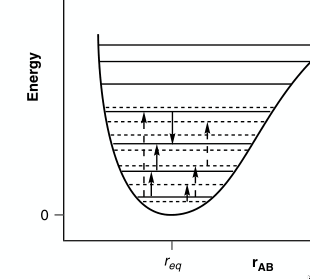
\includegraphics[width=0.5\textwidth]{chem-bond}
		\caption{Typical potential energy of a chemical bond}
		\label{fig:chem-bond}
	\end{figure}

	Everything will be assumed to be described using classical mechanics.
	This is valid when dealing with conformational transitions.
	So all variables are continuous.
	Using this assumption light absorption and a chemical reactions cannot be described.
	The potential energy surface used to describe an unbreakable bond can be seen in figure \ref{fig:chem-bond}.
	When close to the minimum the well can be assumed symmetric, but with some asymmetry later: the left part is steeper.
	An approximation for these potential energy is built into the force field.
	The potential energy surface can be reconstructed using vibrational spectroscopy and then it is reconstructed using a mathematical model.
	Using a Taylor expansion the potential energy is approximated at point $r$ by taking the value at the equilibrium and then constructing all the corrections.
	The first one is the first derivative at the value at equilibrium multiplied by the distance.
	Then for the second correction the second derivative and so on.
	If the potential is symmetric the first derivative is $0$, as it happens near the equilibrium.
	So the first correction can be neglected.
	Also the third order term is either $0$ because the third derivative is $0$ if the minimum is really shallow.
	This term is really small if $r$ is really close to the equilibrium so it can be neglected.

	\begin{align*}
		U(r)&=U(r_{eq}) + \frac{dU}{dr}|_{r=r_{eq}}(r-r_{eq})+\frac{1}{2!}\frac{d^2U}{dr^2}|_{r=r_{eq}}(r-r_{eq}^2)+\frac{1}{3!}\frac{d^3U}{dr^3}|_{r=r_{eq}}(r-r_{eq}^3)+\cdots\\
		U(r)&=U(r_{eq}) + \xcancel{\frac{dU}{dr}|_{r=r_{eq}}(r-r_{eq}})+\frac{1}{2!}\frac{d^2U}{dr^2}|_{r=r_{eq}}(r-r_{eq}^2)+\xcancel{\frac{1}{3!}\frac{d^3U}{dr^3}|_{r=r_{eq}}(r-r_{eq}^3)}+\cdots\\
	\end{align*}

	So that in the end the typical harmonic potential is obtained.

	$$U(r_{AB}) = \frac{1}{2}k_{AB}(r_{AB}-r_{AB,eq})^2$$

	The constant $k$ is related to the second derivative with respect to the distance.
	The distances and the $k$ constants are labelled with $A$ and $B$, which stand for the fact that this interaction has to be described for each couple of atom.
	Transferability of these parameter is an issue: using a particular force field then the parameters cannot be used for another.
	So each force field will come with its own set of parameters.

		\subsubsection{Anharmonic force constant}
		Considering that the shape is not completely symmetric the third order term can be inserted because it can be important.
		This introduces an asymmetry in the system: an anharmonic force constant.

		$$U(r_{AB}) = \frac{1}{2}[k_{AB}+k^{(3)}_{AB}(r_{AB}-r_{AB, eq})](r_{AB}-r_{AB, eq})^2$$

		\subsubsection{Quartic correction}
		Also the fourth order term can be inserted.

		$$U(r_{AB}) = \frac{1}{2}[k_{AB}+k^{(3)}_{AB}(r_{AB}-r_{AB, eq}) + k^{(4)}_{AB}(r_{AB}-r_{AB,eq})^2](r_{AB}-r_{AB, eq})^2$$

		\subsubsection{Morse potential}
		The Morse potential is used in implicit solvent simulation and uses the exponential because it can describe screen interaction that happens with implicit solvent.
		The exponential is quite expensive for a computer to compute.
		It is useful also for soft-systems or coarse grained systems.

		$$U(r_{AB}) = D_{AB}[1-e^{-\alpha_{AB}(r_AB-r_{AB,eq})^2}]$$

\section{Valence angle bending}
Chemical bonds are not described only by strings and beads but also bending of the bonds can happen.
These are valence angle bending, like the one in figure \ref{fig:valence-angle-bending}.

\begin{figure}[H]
	\centering
	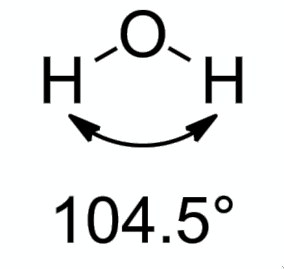
\includegraphics[width=0.3\textwidth]{valence-angle-bending}
	\caption{A valence angle}
	\label{fig:valence-angle-bending}
\end{figure}

These bonds cannot be broken during a classical molecular dynamic simulation.
In order to describe them a Taylor expansion introducing an equilibrium angle is built.
The first order term is not considered as it will be equal to $0$.
Then the second introduces the harmonic and the third for the anharmonic one, in principle also the quartic correction could be added.
This formula is similar to the previous one but all the constant have to be described between each triplet of atoms.

$$U(\theta_{ABC}) = \frac{1}{2}[k_{ABC}+k^{(3)}_{ABC}(\theta_{ABC}-\theta_{ABC,eq})+k^{(4)}_{ABC}(\theta_{ABC}-\theta_{ABC,eq})^2+\cdots](\theta_{ABC}-\theta_{ABC, eq})^2$$

	\subsection{Multiple minima}
	There is another problem with valence angle bending: angles are not varying continuously: the Taylor expansion is good if the angles are not varying to much.
	If the angles invert the Taylor expansion cannot take track of it.
	In order to take this into account the potential energy is built using a Fourier expansion.
	A Fourier expansion introduces a periodic function like $\cos$ that contains oscillations in a period, allowing to model any possible periodic potential.
	Since the angles are being considered the potential is periodic.
	So in the parametrization of the angle bending interaction the Fourier term is introduced, labelling terms with the value $j$.
	So the amplitude, the value that multiplies each Fourier component is decreasing with $j$ and a cut-off of the given value of $j$ is given.
	In this case only low-frequency component are considered.

	$$U(\theta_{ABC}) = \sum\limits_{\{j\}_{ABC}}k^{fourier}_{j,ABC}[1+\cos(j\theta_{ABC}+\psi_j)]$$

	Where the amplitude:

	$$k_{j, ABC}^{fourier} = \frac{2k^{harmonic}_{ABC}}{j^2}$$

	Dividing by $j^2$ makes the contribution smaller for higher $j$.

\section{Torsions}
In order to describe torsion $4$ atoms bonded by subsequent bonds are considered $A->B->C->D$, like if figure \ref{fig:torsions}.

\begin{figure}[H]
	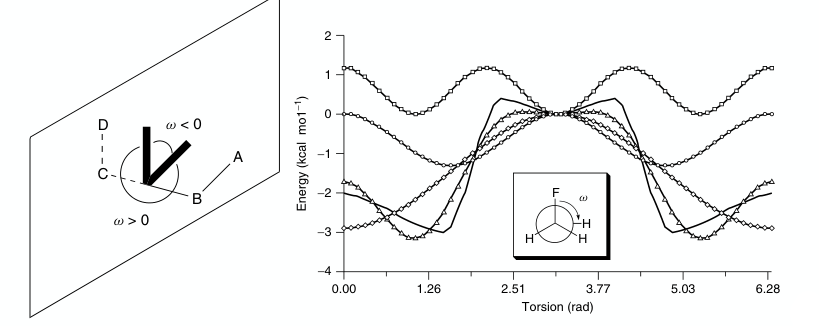
\includegraphics[width=\textwidth]{torsions}
	\caption{An example of torsion}
	\label{fig:torsions}
\end{figure}

In this case two planes $ABC$ and $BCD$ are built and the angle $\omega$ between two plane is built.
If they are on the same plane the angle is $0$.
So an angle $\omega$ is computed to describe the torsion that is around the bond $B->C$.
In order to compute the angle the perpendicular vectors between the planes is computed and the angle between these two vector is $\omega$.
In this case the harmonic oscillation and the Taylor expansion are not used but the Fourier expansion and the periodic potential is used.
This is because the value of the energy will be the same after a rotation.
In principle torsions will be explored during a simulation.
All the possible groups with permutations and repetitions of $4$ atoms need to be considered to parametrize torsions.

$$U(\omega_{ABCD}) = \frac{1}{2}\sum\limits_{\{j\}_{ABCD}}V_{j,ABCD}[1+(-1)^{j+1}\cos(j\omega_{ABCD}+\psi_{j,ABCD})]$$

	\subsection{Improper torsions}
	Improper torsions happen when the bonds are $A->B->C$ and $B->D$ like in figure \ref{fig:improper-torsions}.

	\begin{figure}[H]
		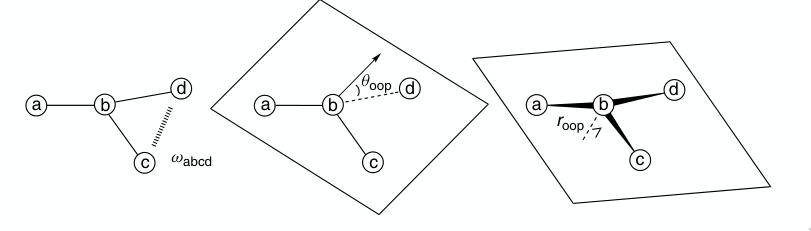
\includegraphics[width=\textwidth]{improper-torsions}
		\caption{An example of improper torsion}
		\label{fig:improper-torsions}
	\end{figure}

	$B$ can be in the same plane of $A, C, D$ or it can pop out.
	In this case two planes are built, usually $ABC$ and $BCD$ and the angle between them will be built.
	The potential will describe the energy of the angle.
	The angle can be described as the out of plane angle $OOP$, obtaining the equation for the plane $ACD$ and how much $B$ is out of that plane.
	Here all possibilities of an atoms connected with other $3$ atoms need to be considered.
	In the case of $sp^2$ the four atoms need to be in a plane.

	$$U(\omega_{ABCD}) = \frac{1}{2}\sum\limits_{\{j\}_{ABCD}}V_{j,ABCD}[1+(-1)^{j+1}\cos(j\omega_{ABCD}+\psi_{j,ABCD})]$$

\section{Van der Waals interactions}
Van der Waals interactions happen whenever two atoms come close to one another without any chemical bond connecting them.
This interaction is called dispersion interaction and depends on the interaction between the electron clouds that become correlated.
Even if electrons are not shared the fluctuation of the electron clouds of an atom will interact with the one of an atom close to it.
Looking at the interaction energy in figure \ref{fig:van-der-waals}.
This can be computed and described by an attraction that goes with the $6$th power of the distance.
This interaction is the Van der Waals interaction.
This attraction is an attractive force and will decrease with the $6$th power of the distance.
Also a repulsion happen.
The repulsion is due to the occupancy of the possible orbitals.
The problem is then Pauli's exclusion principle: whenever two atoms come close the energy level becomes occupied and the atoms cannot come to close to one another.
This is difficult to compute but it can be modelled assuming that is a repulsion with an hard limit.
The energy becomes very high when the distance becomes less than the equilibrium.
If the attraction is modelled with the $6$th power this interaction can be modelled by the $12$th power.
In this case if the distance is too small the energy becomes very high.

\begin{figure}[H]
	\centering
	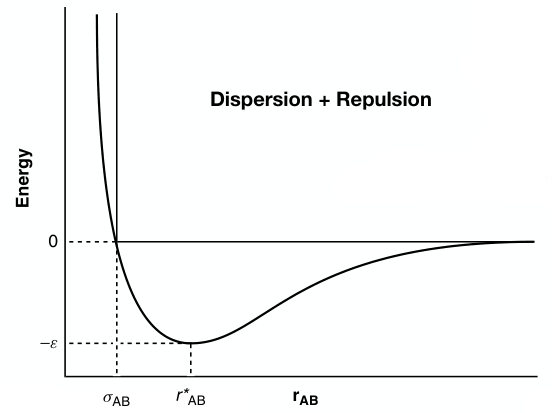
\includegraphics[width=0.5\textwidth]{van-der-waals}
	\caption{Energy of a Van der Waals interaction}
	\label{fig:van-der-waals}
\end{figure}

	\subsection{Lennard-Jones potential}
	The discussion done above lead to the introduction of the Lennard-Jones potential.
	This models Van der Waals interaction using the $6$th power for the dispersion and the repulsion due to Pauli's exclusion principle is modelled by the $12$th power.
	This power is used to make the computation cheap and has no physical basis.
	In this way this formula is obtained:

	\begin{align*}
		U_(r_{AB}) &= \frac{a_{AB}}{r^{12}_{AB}}-\frac{b_{AB}}{r^6_{AB}}=\\
							 &= 4\epsilon_{AB}\biggl[\biggl(\frac{\sigma_{AB}}{r_{AB}}\biggr)^{12}-\biggl(\frac{\sigma_{AB}}{r_{AB}}\biggr)^6\biggr]
	\end{align*}

	And the distance with minimum energy or equilibrium.

	$$r^*_{AB} = 2^{\frac{1}{6}}\sigma_{AB}$$

	And it can be seen how it is a multiple of $\sigma_{AB}$ or the Van der Waals radius, the distance where the value of the energy if exactly equal to $0$.
	$-\epsilon$ is the minimum value of the energy (equilibrium).
	In this way dispersion and repulsion of any couple of atoms can be described.
	A value of $\sigma_{AB}$ have to be introduced for any couple of atom type.

	\subsection{Morse potential}
	The Morse potential and the Hill potential can be used with coarse grained system.
	Dealing only with all-atom simulation these will be rarely used.
	Working in soft-matter simulation these could be used.
	These have the same features of the Lennard-Jones potential.

	$$U(r_{AB}) = D_{AB}[1-e^{-a_{AB}(r_{AB}-r_{AB,eq})^2}]$$

	\subsection{Hill potential}

	$$U(r_{AB}) = \epsilon_{AB}\biggl[\frac{6}{\beta_{AB}-6}e^{\beta_{AB}\frac{1-r_{AB}}{r^*_{AB}}}-\frac{\beta_{AB}}{\beta_{AB}-6}\biggl(\frac{r^*_{AB}}{r_{AB}}\biggr)^6\biggr]$$

	In some force fields $1$-$4$ interactions (successive bonds atoms can be numbered) are reduced by a scaled factor.
	Atom $1$ and $4$ are cose to each other in a proper torsion but attraction and repulsion has been already described by the torsion, so in some force fields, the torsions takes into account the proximity of those atoms.
	So the Van der Waals interactions are excluded for $1$-$4$ atoms as they are already been described by the torsion interaction.


\section{Electrostatic interactions}
Electrostatic interactions, together with Van der Waals one are two kind of non-bonded interactions.
Moreover interactions between molecules that might be charged or that can be polar.
The distribution of charges need to be described.
In principle a multiple expansion should be performed: the cloud of positive and negative charges should be described by using given shapes of the clouds.
And each molecule should be described and all the molecules should be described by these multiple expansion and they should be multiplied as matrix.

$$U_{AB} = \vec{M}^{(A)}V^{(B)}$$

Now, summing over all molecules:

$$U_{AB} = \sum\limits_{A}\sum\limits_{B>A}\vec{M}^{(A)}\vec{V}^{(B)}$$

This is a very costly procedure but accurate.

	\subsection{Point like charges}
	To make the computation easier molecules are represented as point-like partial charges.
	In a chemical molecule partial charges can be assumed that are point-like and are located on the atom.
	The electron cloud is displaced toward the negative cloud and away from the positive one.
	In this way the distribution of charges can be represented by number placed on each atom.
	Once this is done an electric charge is associated with each bead and the Coulomb interaction is used:

	$$U_{AB} = \frac{q_Aq_B}{\epsilon_{AB}r_{AB}}$$

	The dielectric constant is $1$ in the case of explicit solvent, but in the case of the implicit one it will be the one of the solvent.

	\subsection{Dipolar interactions}
	Dipolar interaction can be included when considering electrostatic forces.
	These formulae are mostly used in corse grained models.
	Because in that case the approximation of single charges on a bead cannot be made and dipoles are considered.
	In this case a functional form and the parameters need to be included.
	$\mu$ is the dipole of two molecules.
	Then there is the dielectric constant, the cube of the distance and the cosine term represent the orientation of the two dipoles.

	$$U_{AB/CD} = \frac{\mu_{AB}\mu_{CD}}{\epsilon_{AB/CD}r^3_{AB/CD}}(\cos\chi_{AB/CD}-3\cos\alpha_{AB}\cos\alpha_{CD})$$

	\begin{figure}[H]
		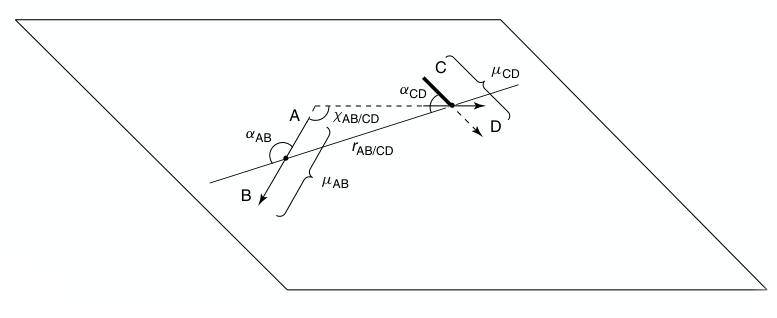
\includegraphics[width=\textwidth]{dipolar-interactions}
		\caption{An example of a dipolar interaction}
		\label{fig:dipolar-interactions}
	\end{figure}

	\subsection{Dielectric constants}

	$$U_{AB} = \frac{q_Aq_B}{\epsilon_{AB}r_{AB}}$$

	The dielectric constant can assume different values.
	If they are connected by a chemical bond or if there is a valence angle between the atoms the dielectric constant if $\infty$ and the interaction is not computed as it is already taken into account by other terms.
	In several force field a factor of $2$ is added for $1$-$4$ interaction.
	In the last case the value depend on the force field.

	$$\epsilon_{AB} = \begin{cases}\infty&\text{ if }A\land B\text{are 1,2- or 1,3-related}\\3.0&\text{ if }A\land B\text{are 1,4-related}\\1.5&\text{otherwise}\end{cases}$$

\section{Cross terms}
There are also cross terms: angle bending and bond stretching and other movement are not independent: all the possible degrees of freedom should be considered together.
This is done only by some force fields.

\begin{align*}
	U(\vec{q}) = &U(\vec{q}_{eq}) + \sum\limits_{i=1}^{3N-6}(q_i-q_{i,eq})\frac{\partial U}{\partial q_i}|_{\vec{q}=\vec{q}_{eq}} + \\
							 &+\frac{1}{2!}\sum\limits_{i=1}^{3N-6}\sum\limits_{j=1}^{3N-6}(q_i-q_{i.eq})(q_j-q_{j,eq})\frac{\partial^2 U}{\partial q_i\partial q_j}|_{\vec{q}=\vec{q}_{eq}} +\\
							 &=\frac{1}{3!}\sum\limits_{i=1}^{3N-6}\sum\limits_{j=1}^{3N-6}\sum\limits_{k=1}^{3N-6}(q_i-q_{i,eq})(q_j-q_{j.eq})(q_k-q_{k,eq})\frac{\partial^3 U}{\partial q_i\partial q_j\partial q_k}|_{\vec{q}=\vec{q}_{eq}} + \cdots
\end{align*}

This is done by starting from a Lagrangian describing all the interaction and compute all the terms.
In practice everything is done without considering them.

$$U(r_{AB}, \theta_{ABC}) = \frac{1}{2}k_{AB,ACB}(r_{AB}-r_{AB, eq})(\theta_{ABC}-\theta_{ABC, eq})$$

\section{Parametrization}
All the interactions need a large set of parameters.
The number of parameters increases with the number of atoms $N$:

$$p = N + (N-1)+(N-2)+\cdots = N\frac{N+1}{2}$$

In order to obtain these parameters data from experiments are used.
This is the reason why the force-field are semi-empirical.
To do so the results of the experiments are compared from the results of simulations.
Then the penalty function:

$$Z = \biggl[\sum\limits_{i}^{observables}\sum\limits_{j}^{occurrences}\frac{(calc_{i,j}-expt_{i,j})^2}{w_i^2}\biggr]^{\frac{1}{2}}$$

Sums over all the data from all the observables and all possibilities.
Then all the observable are measured and are compared with the simulation result.
Then the square is taken to not compensate the error and it is divided by a weight.
This penalty function is minimized changing the parameters until some reasonable compromise is obtained.
The more experimental data is obtained the more accurate the description.
This is the reason for the constant update of the force fields.
A way to reduce the number of parameters is to employ a strategy so that a parameter to each atom is computed and then it is computed the interaction between two atoms:

\begin{align*}
	\sigma_{AB} &= \sigma_A+\sigma_B\\
	\epsilon_{AB} &= (\epsilon_A\epsilon_B)^{\frac{1}{2}}
\end{align*}

\section{Force field energies}
In molecules the ground state of one molecule is different from the ground state of another.
Molecules can have different states and when they come in contact the ground state have to be taken into account.
So parametrizing the force field is very complicated.

	\subsection{Geometry optimization}
	Once the force fields are obtained some atoms can be missing from the model and have to be included by hand.
	Sometimes it may happen that two atoms are too close to each other and by using the potential energy it can be high leading to high forces, causing the atom that experience them to be kicked out.
	So the simulation will explode.
	In order to avoid this a geometry optimization is done to obtain the parameters or to minimize so to avoid high forces values at the start of a simulation.
	When starting a simulation the system will be at an energy value which be greater than the equilibrium.
	The gradient of the energy is computed and the system is moved toward the minimum energy.
	The derivative need to be computed of $U$ with respect to each component in the system.

	$$\vec{g}(\vec{q}) = \begin{bmatrix} \frac{\partial U}{\partial q_1} \\ \frac{\partial U}{\partial q_2} \\ \vdots \\ \frac{\partial U}{\partial q_n}\end{bmatrix}$$

	Such that the cost reaches a global minimum $J_{min}(\vec{w})$.

	\subsection{Derivative of the potential function}
	First the derivatives need to be computed.
	All the potentials are given in term of the mutual distance of two atoms.
	So, considering $x$ the coordinates of a point:

	$$\frac{\partial U}{\partial x_A} = \sum\limits_{i\in A}\frac{\partial U}{\partial r_{Ai}}\frac{\partial r_{Ai}}{\partial x_A}$$

	Taking the derivative of this:

	$$U(r_{AB}) = \frac{1}{2}[k_{AB}+k_{AB}^{(3)}(r_{AB}-r_{AB, eq}) + k_{AB}^{(4)}(r_{AB}-r_{AB, eq})^2](r_{AB}-r_{AB,eq})^2$$

	With the respect on the distance:

	$$\frac{\partial U}{\partial r_{Ai}} = \frac{1}{2}[2k_{Ai}+3k_{Ai}^{(3)}r_{Ai}-r_{Ai, eq}) + 4k^{(4)}_{Ai}(r_{Ai}-r_{Ai, eq})^2](r_{Ai}-r_{Ai, eq})$$

	In order to take the derivative with respect to $r$ with respect to $x$ need to be known:

	$$\frac{\partial r_{Ai}}{\partial x_A} = \frac{x_A-x_i}{\sqrt{(x_A-x_i)^2+(y_A-y_i)^2+(z_A-z_i)^2}}$$

	Then this formula can plugged in according to the chain rule.

		\subsubsection{Newton-Raphson}
		To perform the minimization as an iterative procedure, the Newton-Raphson to find a local minimum is employed.
		Here $(n)$ refers to the iteration.
		This allow to obtain iteration $k+1$ starting from iteration $k$ and is a Taylor expansion of coordinates at iteration $k$:

		$$U(\vec{q}^{(k+1)}) = U(\vec{q}^{(k)}) + (\vec{q}^{(k+1)} -\vec{q}^{(k)})\vec{g}^{(k)} + \frac{1}{2}(\vec{q}^{(k+1)}-\vec{q}^{(k)})H^{(k)}(\vec{q}^{(k+1)}-\vec{q}^{(k)})$$

		This is done to find eventually the coordinates at iteration $k+1$ which are unknown.
		Where $H$ is the Hessian matrix built:

		$$H_{ij}^{(k)} = \frac{\partial^2 U}{\partial q_i\partial q_j}|_{\vec{q}=\vec{q}^{(k)}}$$

		Everything is computed from a Taylor expansion from coordinates at iteration $k$.
		And:

		$$\frac{\partial U(\vec{q}^{(k+1)})}{\partial q_i^{(k+1)}} = \frac{\partial \vec{q}^{(k+1)}}{\partial q_i^{(k+1)}}\vec{g}^{(k)}+ \frac{1}{2}\frac{\partial \vec{q}^{(k+1)}}{\partial q_i^{(k+1)}}H^{(k)}(\vec{q}^{(k+1)}-\vec{q}^{(k)})+\frac{1}{2}(\vec{q}^{(k+1)}-\vec{q}^{(k)})H^{(k)}\frac{\partial \vec{q}^{(k+1)}}{\partial q_i^{(k+1)}}$$

		This formula tells that:

		$$\vec{g}_i^{(k+1)} = \vec{g}_i^{(k)} + [H^{(k)}(\vec{q}^{(k+1)}-\vec{q}^{(k)})]_i$$

		Where at the end it should be obtained a stationary condition, where the system does not change after an iteration:

		$$\vec{0} = \vec{g}^{(k)} + H^{(k)}(\vec{q}^{(k+1)}-\vec{q}^{(k)})\Rightarrow \vec{q}^{(k+1)} = \vec{q}^{(k)} - [H^{(k)}]^{-1}\vec{g}^{(k)}$$

		Because the starting point was a Taylor expansion the new coordinates will not be exact, and so other iterations will be needed.
		This process is repeated until convergence is reached, choosing a given tolerance on $\vec{0}$.

	\subsection{Types of force fields}
	Force fields can be categorized as:

	\begin{multicols}{2}
		\begin{itemize}
			\item All atoms: one atom corresponds to one bead.
			\item More atoms: more atoms correspond to one bead.
			\item Corse grained: groups of atoms correspond to one bead.
			\item Polarizable force fields: point charges are variables.
		\end{itemize}
	\end{multicols}

	As a golden rule parameters from different force fields should never be mixed.
